% Created by tikzDevice version 0.12.6 on 2026-08-03 03:41:19
% !TEX encoding = UTF-8 Unicode
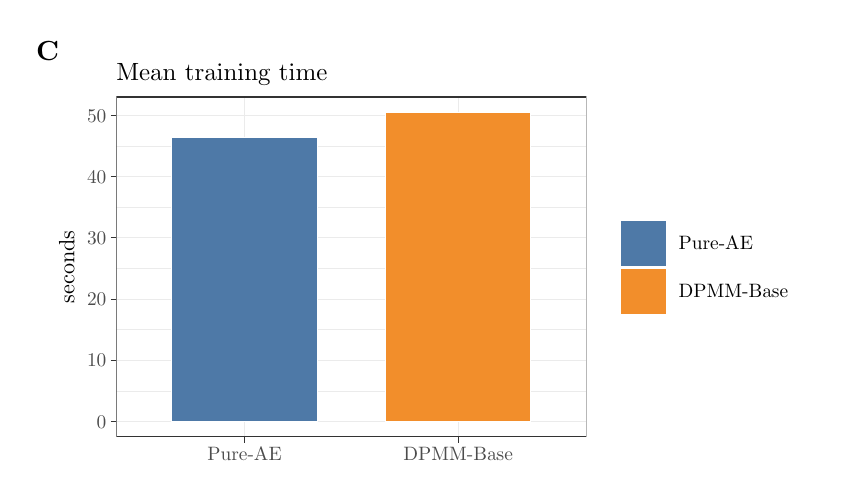
\begin{tikzpicture}[x=1pt,y=1pt]
\definecolor{fillColor}{RGB}{255,255,255}
\path[use as bounding box,fill=fillColor,fill opacity=0.00] (0,0) rectangle (283.84,161.83);
\begin{scope}
\path[clip] (  1.05,  1.74) rectangle (282.80,160.09);
\definecolor{drawColor}{RGB}{255,255,255}
\definecolor{fillColor}{RGB}{255,255,255}

\path[draw=drawColor,line width= 0.4pt,line join=round,line cap=round,fill=fillColor] (  1.05,  1.74) rectangle (282.80,160.09);
\end{scope}
\begin{scope}
\path[clip] ( 32.04, 13.93) rectangle (201.87,136.79);
\definecolor{fillColor}{RGB}{255,255,255}

\path[fill=fillColor] ( 32.04, 13.93) rectangle (201.87,136.79);
\definecolor{drawColor}{gray}{0.92}

\path[draw=drawColor,line width= 0.2pt,line join=round] ( 32.04, 30.58) --
	(201.87, 30.58);

\path[draw=drawColor,line width= 0.2pt,line join=round] ( 32.04, 52.69) --
	(201.87, 52.69);

\path[draw=drawColor,line width= 0.2pt,line join=round] ( 32.04, 74.81) --
	(201.87, 74.81);

\path[draw=drawColor,line width= 0.2pt,line join=round] ( 32.04, 96.93) --
	(201.87, 96.93);

\path[draw=drawColor,line width= 0.2pt,line join=round] ( 32.04,119.04) --
	(201.87,119.04);

\path[draw=drawColor,line width= 0.4pt,line join=round] ( 32.04, 19.52) --
	(201.87, 19.52);

\path[draw=drawColor,line width= 0.4pt,line join=round] ( 32.04, 41.63) --
	(201.87, 41.63);

\path[draw=drawColor,line width= 0.4pt,line join=round] ( 32.04, 63.75) --
	(201.87, 63.75);

\path[draw=drawColor,line width= 0.4pt,line join=round] ( 32.04, 85.87) --
	(201.87, 85.87);

\path[draw=drawColor,line width= 0.4pt,line join=round] ( 32.04,107.98) --
	(201.87,107.98);

\path[draw=drawColor,line width= 0.4pt,line join=round] ( 32.04,130.10) --
	(201.87,130.10);

\path[draw=drawColor,line width= 0.4pt,line join=round] ( 78.36, 13.93) --
	( 78.36,136.79);

\path[draw=drawColor,line width= 0.4pt,line join=round] (155.55, 13.93) --
	(155.55,136.79);
\definecolor{drawColor}{RGB}{255,255,255}
\definecolor{fillColor}{RGB}{78,121,167}

\path[draw=drawColor,line width= 0.3pt,fill=fillColor] ( 52.11, 19.52) rectangle (104.60,122.14);
\definecolor{fillColor}{RGB}{242,142,43}

\path[draw=drawColor,line width= 0.3pt,fill=fillColor] (129.31, 19.52) rectangle (181.80,131.21);
\definecolor{drawColor}{gray}{0.20}

\path[draw=drawColor,line width= 0.4pt,line join=round,line cap=round] ( 32.04, 13.93) rectangle (201.87,136.79);
\end{scope}
\begin{scope}
\path[clip] (  0.00,  0.00) rectangle (283.84,161.83);
\definecolor{drawColor}{gray}{0.30}

\node[text=drawColor,anchor=base east,inner sep=0pt, outer sep=0pt, scale=  0.70] at ( 28.44, 17.11) {0};

\node[text=drawColor,anchor=base east,inner sep=0pt, outer sep=0pt, scale=  0.70] at ( 28.44, 39.22) {10};

\node[text=drawColor,anchor=base east,inner sep=0pt, outer sep=0pt, scale=  0.70] at ( 28.44, 61.34) {20};

\node[text=drawColor,anchor=base east,inner sep=0pt, outer sep=0pt, scale=  0.70] at ( 28.44, 83.46) {30};

\node[text=drawColor,anchor=base east,inner sep=0pt, outer sep=0pt, scale=  0.70] at ( 28.44,105.57) {40};

\node[text=drawColor,anchor=base east,inner sep=0pt, outer sep=0pt, scale=  0.70] at ( 28.44,127.69) {50};
\end{scope}
\begin{scope}
\path[clip] (  0.00,  0.00) rectangle (283.84,161.83);
\definecolor{drawColor}{gray}{0.20}

\path[draw=drawColor,line width= 0.4pt,line join=round] ( 30.04, 19.52) --
	( 32.04, 19.52);

\path[draw=drawColor,line width= 0.4pt,line join=round] ( 30.04, 41.63) --
	( 32.04, 41.63);

\path[draw=drawColor,line width= 0.4pt,line join=round] ( 30.04, 63.75) --
	( 32.04, 63.75);

\path[draw=drawColor,line width= 0.4pt,line join=round] ( 30.04, 85.87) --
	( 32.04, 85.87);

\path[draw=drawColor,line width= 0.4pt,line join=round] ( 30.04,107.98) --
	( 32.04,107.98);

\path[draw=drawColor,line width= 0.4pt,line join=round] ( 30.04,130.10) --
	( 32.04,130.10);
\end{scope}
\begin{scope}
\path[clip] (  0.00,  0.00) rectangle (283.84,161.83);
\definecolor{drawColor}{gray}{0.20}

\path[draw=drawColor,line width= 0.4pt,line join=round] ( 78.36, 11.93) --
	( 78.36, 13.93);

\path[draw=drawColor,line width= 0.4pt,line join=round] (155.55, 11.93) --
	(155.55, 13.93);
\end{scope}
\begin{scope}
\path[clip] (  0.00,  0.00) rectangle (283.84,161.83);
\definecolor{drawColor}{gray}{0.30}

\node[text=drawColor,anchor=base,inner sep=0pt, outer sep=0pt, scale=  0.70] at ( 78.36,  5.51) {Pure-AE};

\node[text=drawColor,anchor=base,inner sep=0pt, outer sep=0pt, scale=  0.70] at (155.55,  5.51) {DPMM-Base};
\end{scope}
\begin{scope}
\path[clip] (  0.00,  0.00) rectangle (283.84,161.83);
\definecolor{drawColor}{RGB}{0,0,0}

\node[text=drawColor,rotate= 90.00,anchor=base,inner sep=0pt, outer sep=0pt, scale=  0.80] at ( 16.86, 75.36) {seconds};
\end{scope}
\begin{scope}
\path[clip] (  0.00,  0.00) rectangle (283.84,161.83);
\definecolor{fillColor}{RGB}{255,255,255}

\path[fill=fillColor] (209.87, 54.02) rectangle (280.80, 96.71);
\end{scope}
\begin{scope}
\path[clip] (  0.00,  0.00) rectangle (283.84,161.83);
\definecolor{fillColor}{RGB}{255,255,255}

\path[fill=fillColor] (213.87, 75.36) rectangle (231.22, 92.71);
\definecolor{drawColor}{RGB}{255,255,255}
\definecolor{fillColor}{RGB}{78,121,167}

\path[draw=drawColor,line width= 0.3pt,fill=fillColor] (214.23, 75.72) rectangle (230.86, 92.35);
\end{scope}
\begin{scope}
\path[clip] (  0.00,  0.00) rectangle (283.84,161.83);
\definecolor{fillColor}{RGB}{255,255,255}

\path[fill=fillColor] (213.87, 58.02) rectangle (231.22, 75.36);
\definecolor{drawColor}{RGB}{255,255,255}
\definecolor{fillColor}{RGB}{242,142,43}

\path[draw=drawColor,line width= 0.3pt,fill=fillColor] (214.23, 58.37) rectangle (230.86, 75.01);
\end{scope}
\begin{scope}
\path[clip] (  0.00,  0.00) rectangle (283.84,161.83);
\definecolor{drawColor}{RGB}{0,0,0}

\node[text=drawColor,anchor=base west,inner sep=0pt, outer sep=0pt, scale=  0.70] at (235.22, 81.62) {Pure-AE};
\end{scope}
\begin{scope}
\path[clip] (  0.00,  0.00) rectangle (283.84,161.83);
\definecolor{drawColor}{RGB}{0,0,0}

\node[text=drawColor,anchor=base west,inner sep=0pt, outer sep=0pt, scale=  0.70] at (235.22, 64.28) {DPMM-Base};
\end{scope}
\begin{scope}
\path[clip] (  0.00,  0.00) rectangle (283.84,161.83);
\definecolor{drawColor}{RGB}{0,0,0}

\node[text=drawColor,anchor=base west,inner sep=0pt, outer sep=0pt, scale=  0.90] at ( 32.04,142.78) {Mean training time};
\end{scope}
\begin{scope}
\path[clip] (  0.00,  0.00) rectangle (283.84,161.83);
\definecolor{drawColor}{RGB}{0,0,0}

\node[text=drawColor,anchor=base,inner sep=0pt, outer sep=0pt, scale=  1.00] at (  7.20,150.08) {\bfseries C};
\end{scope}
\end{tikzpicture}
